\documentclass[11pt]{article}
\title{\textbf{CS 296: Lab 7}}
\author{Siddhartha Dutta \\ 120040005 \and Gangadhar KV \\ 120050078 \and Sai Krishna Kethan \\ 120050065}
\date{March 1, 2014}
\usepackage{graphicx}
\begin{document}

\maketitle

\section{Timing}
\subsection{Analyzing results of Lab 5}

\begin{figure}[ht!]
\centering
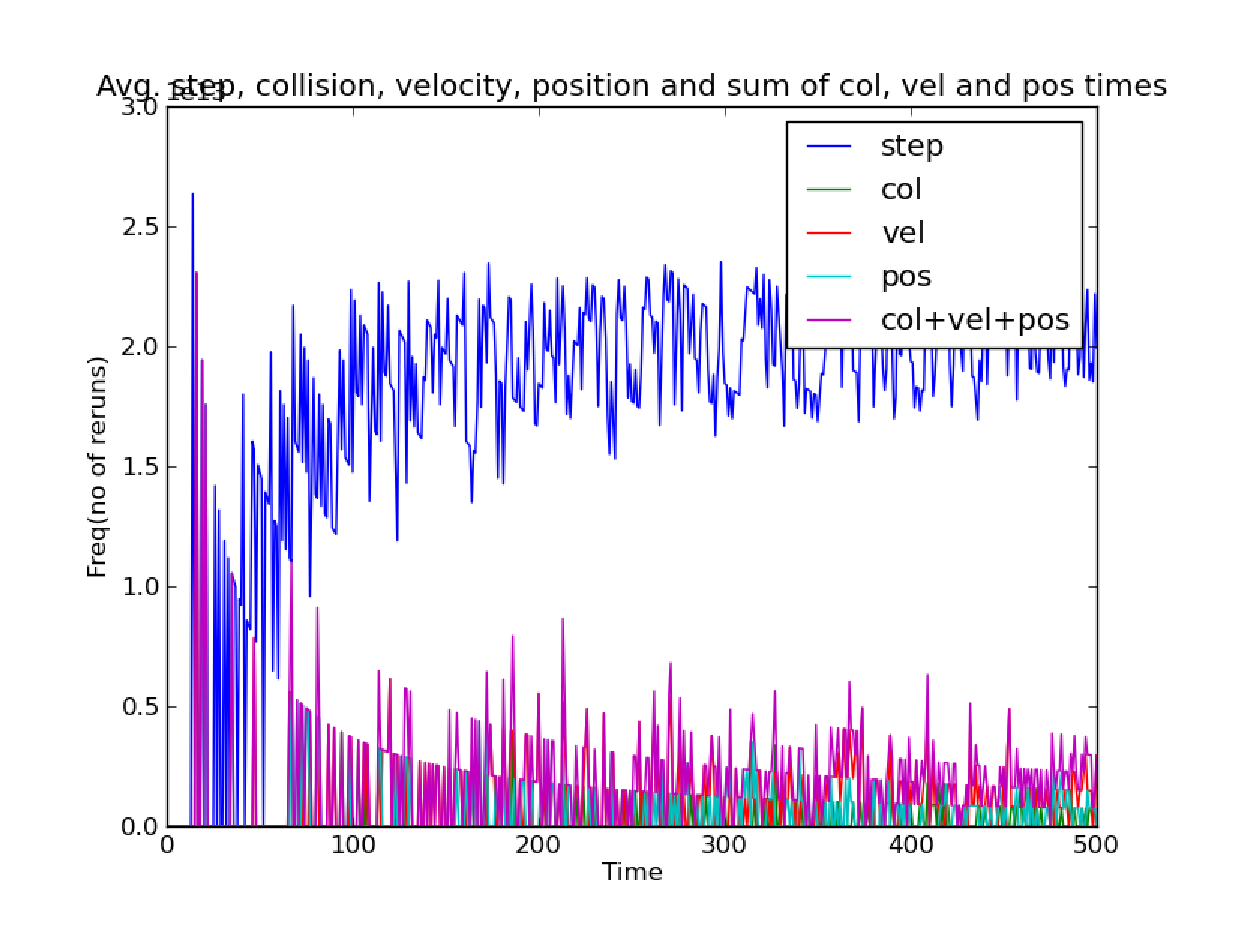
\includegraphics[width=90mm]{g32_plot02.eps}
\caption{Avg. Step Time vs Iteration Values}
\label{overflow}
\end{figure}

In the above graph, we observe that the average step time in the beginning is quite high. As the number of iterations increases, the average step time keeps decreasing. There is a sharp fall after around 30 iterations. But after 50 iterations, the step time increases slowly till around 150 and then levels off. The above graph shows data for 500 iterations. 

This can be explained if we realize that initially the wheels and rods are all still. As the wheel begins to move, forces are exerted upon the revolute joints of various rods. Since in a given loop greater part of the time is spent on resolving collisions, the start time is quite high as various velocity and position calculations have to be made to get things moving. 

As time passes on approximate solutions to equations are obtained and much lesser time and iterations of position and velocity solver is required to obtain fine tuned solutions. This explains the drop in time. There are frequent spikes in the graph due to the continuos calls made to the solver when piston reaches an end of the oscillation. The graph levels off and becomes regular with time since most bodies begin to move in a definite order and the same kind of motions are repeated after a certain period.

In every loop "Step" in B2World \cite{ref2} in called. A solver is used in collision time, velocity time and position time. Box2D also uses a constraint solver for solving constraints. The constraint solver solves all the constraints in the simulation, one at a time. Altough single constraint can be solved perfectly, when we solve one constraint, we slightly disrupt other constraints. Therefore to get a good solution, we need to iterate over all constraints a number of times. Thus, multiple iterations for position and velocity are needed.

\begin{figure}[ht!]
\centering
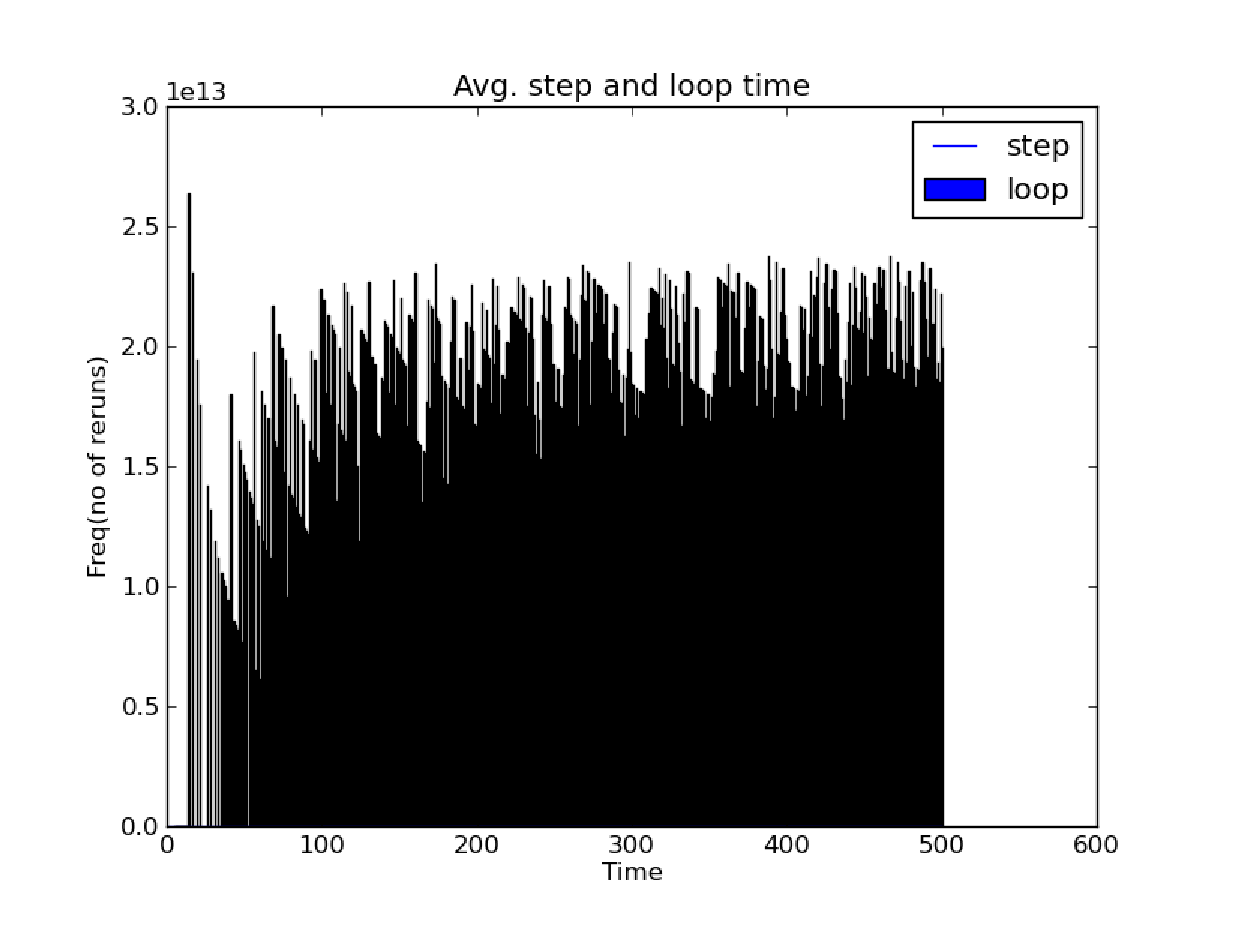
\includegraphics[width=90mm]{g32_plot01.eps}
\caption{Total loop time}
\label{overflow}
\end{figure}

This graph reiterates the observations made earlier.The total loop time is completely linear to the number of iterations. This is in concurrence with the fact that the average step time becomes constant.

\begin{figure}[ht!]
\centering
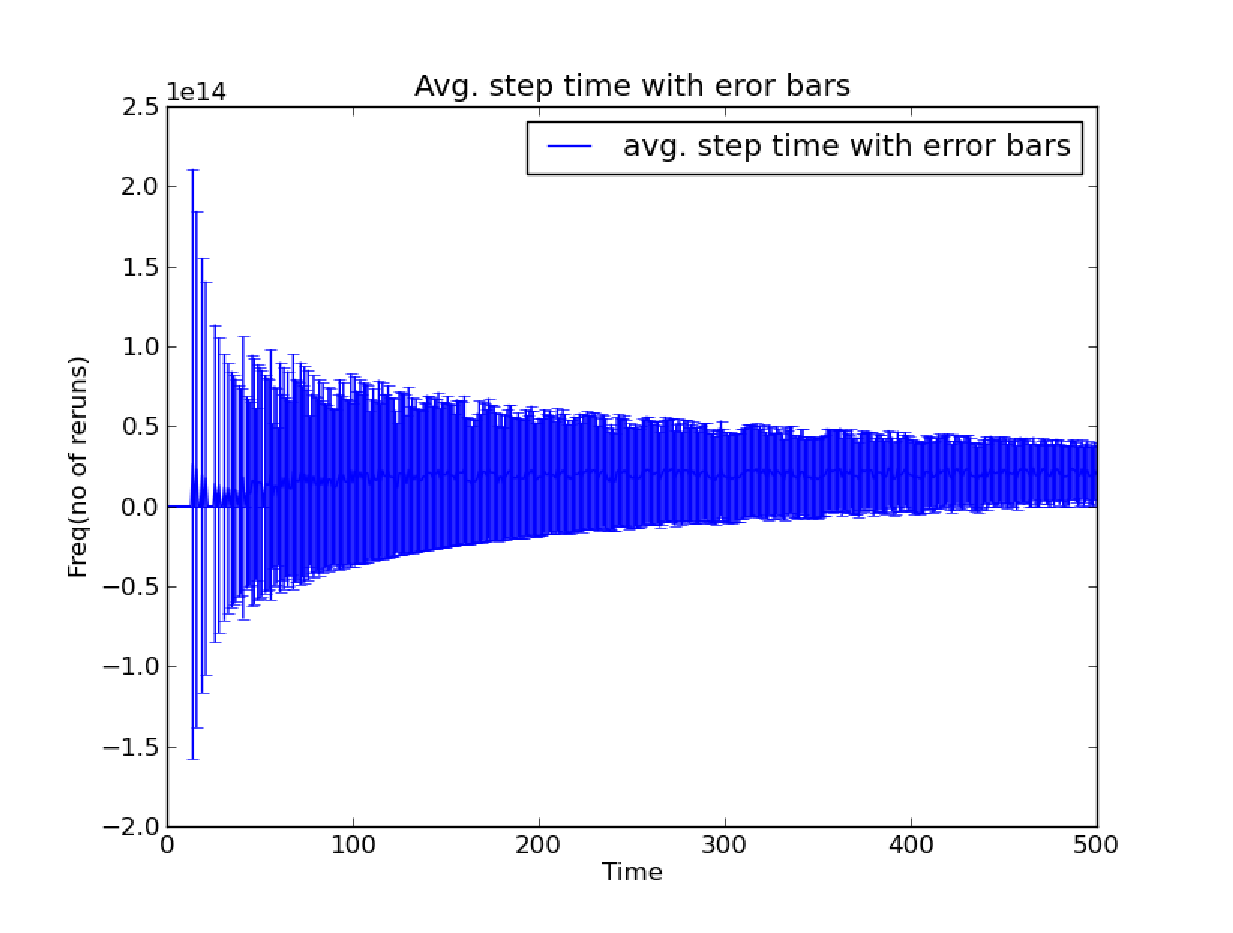
\includegraphics[width=90mm]{g32_plot03.eps}
\caption{Avg. Step Time vs Iteration Values with error bars}
\label{overflow}
\end{figure}

The above plot represents average step time and y-error bars. As can be clearly observed, the difference between the maximum and minimum values is very large. The values are taken within 50 system iterations(very close times for processing). The differences can be attributed to system processes. The error range is intitially a bit high when step times are high but decreases gradually as the step time levels off.

\subsection{Time vs gettimeofday()}
Time writes to standard error giving various statistics regarding the running time of the program. These statistics consist of 
\begin{enumerate}
\item the elapsed real time between invocation and termination, 
% \item the user CPU time (the sum of the tms_utime and tms_cutime values in a struct tms), and 
% \item the system CPU time (the sum of the tms_stime and tms_cstime values in a struct tms).
\end{enumerate}
Time command measures the whole program execution time, including the time it takes to load the binary and all its libraries. It also includes the time it takes to clean up everything once the program is finished.

On the other hand, gettimeofday can only work inside the program, that is after it has finished loading (for the initial measurement) and before it is cleaned up (for the final measurement). It gives the exact time required to execute the function.

The function gettimeofday has higher resolution than time: time can return only in seconds while gettimeofday() returns in microseconds.

\subsection{System under heavy loading}
While running CPU heavy processes, the time increases since smaller processing time is devoted to our process. I tried this by making several codes run in different terminals.

On the other hand while running RAM intensive processes, it waits and tries to kill other processes. Since the processor may be idle all this while, there's no significant change in time. 

\section{Profiling}
\subsection{Introduction}

Profiling \cite{ref1} is a form of dynamic program analysis that measures, the space (memory) or time complexity of a program, the usage of particular instructions, or frequency and duration of function calls. The most common use of profiling information is to aid program optimization.

\subsection{Optimization}
Turning on optimization flags makes the compiler attempt to improve the performance and/or code size at the expense of compilation time and possibly the ability to debug the program. The compiler performs optimization based on the knowledge it has of the program. Optimization levels -O2 and above, in particular, enable unit-at-a-time mode, which allows the compiler to consider information gained from later functions in the file when compiling a function. Compiling multiple files at once to a single output file in unit-at-a-time mode allows the compiler to use information gained from all of the files when compiling each of them. An example of optimization is inlining the functions.

For what follows, the profiler was run over 1000 iterations.

\subsection{Release Build}


\begin{figure}[ht!]
\centering
\includegraphics[width=150mm]{g32_release_prof.eps}
\caption{Call graph for Release}
\label{overflow}
\end{figure}

\begin{figure}[ht!]
\centering
\includegraphics[width=150mm]{release.eps}
\caption{Call graph for Release}
\label{overflow}
\end{figure}

The release build is faster than the debug build since it uses optimization. Also it eliminates debugging information since it meant for the end-user. We used the O3 flag for compilation and used cmake -DCMAKE\_BUILD\_TYPE=Release for building.
By observing perf report, we conclude that Position Constraint Solver and velocity constraint solver takes more time. But we can't optimise them any further as they are key for constraints.We observe that b2Vec2 takes significantly more time.This reveals that time taking processes are very less in our simulation. 
\bibliographystyle{plain}
\bibliography{g32_prof_report}




\end{document}
